% !TEX root = ../tex/5-1.tex
% 第5章：本文は青、補足は緑
\newcommand{\asmain}{%
    \setbeamercolor{frametitle}{fg=white,bg=main}%
    \setbeamercolor{structure}{fg=main}%
    \setbeamercolor{itemize item}{fg=main}%
    \setbeamercolor{itemize subitem}{fg=main}%
    \setbeamercolor{enumerate item}{fg=main}%
}
\newcommand{\assuppl}{%
    \setbeamercolor{frametitle}{fg=white,bg=examplecol}%
    \setbeamercolor{structure}{fg=examplecol}%
    \setbeamercolor{itemize item}{fg=examplecol}%
    \setbeamercolor{itemize subitem}{fg=examplecol}%
    \setbeamercolor{enumerate item}{fg=examplecol}%
}
% フレームタイトルの「補足」だけを□で囲む
\newcommand{\supplmark}{%
    \setlength{\fboxsep}{1.5pt}%
    \setlength{\fboxrule}{0.7pt}%
    \fbox{\textbf{補足}}%
}
\asmain


%=============================================
\begin{frame}{第4章から第5章へ}
    \begin{block}{ここまで（第4章 Score SDE）}
        スコア$\nabla_{\bm{x}}\log p_t$を学び、\\
        逆時間SDE／PF-ODEの速度場を組み立てて生成する。
    \end{block}
    \begin{block}{ここから（第5章 Flow Matching）}
        同じ確率流でも、速度場$\bm{v}_t$を\textbf{直接}学ぶ道がある。\\
        まず離散の正規化フローから連続のNeural ODEへ進み、\\
        次節でFlow Matchingの枠組みに入る。
    \end{block}
\end{frame}
%=============================================
\asmain
\begin{frame}{図5.1：Score SDE と Flow Matchingの対応}
    \centering
    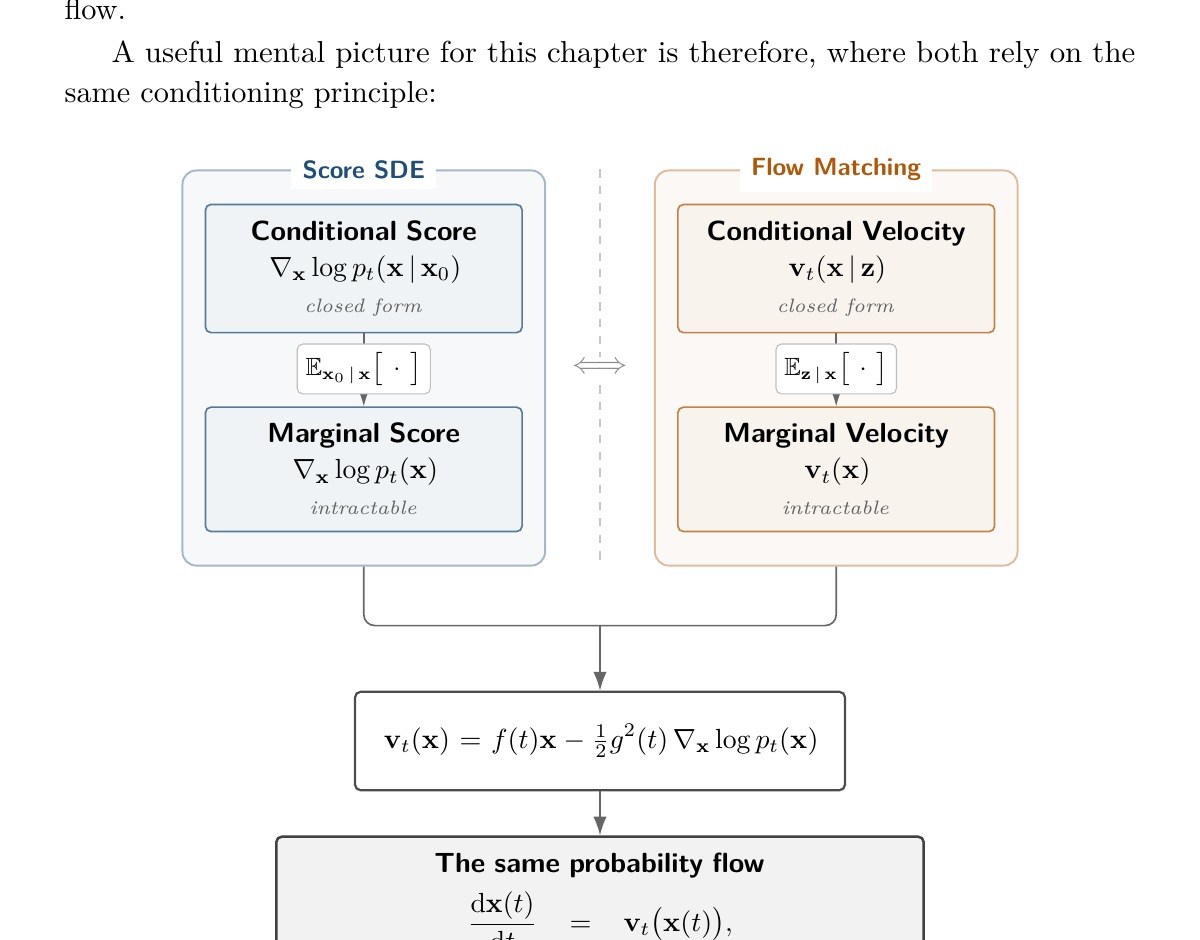
\includegraphics[width=\textwidth,height=0.62\textheight,keepaspectratio]{fig-5-1.jpg}
    \vfill
    \footnotesize
    条件付きの閉じた教師$\to$期待で周辺へ。\\
    拡散経路ではスコアから速度が決まり、FMはその速度を直接回帰する。
\end{frame}
%=============================================
\assuppl
\begin{frame}{\supplmark：図5.1の読み方}
    \begin{columns}[T,onlytextwidth]
        \begin{column}{0.48\textwidth}
            \begin{exampleblock}{Score SDE}
                条件付きスコア（閉じた形）\\
                $\;\to\;$周辺スコア（扱いにくい）\\
                $\;\to\;$PF-ODE速度へ変換
            \end{exampleblock}
        \end{column}
        \begin{column}{0.48\textwidth}
            \begin{exampleblock}{Flow Matching}
                条件付き速度（閉じた形）\\
                $\;\to\;$周辺速度（扱いにくい）\\
                $\;\to\;$同じODEを直接学習
            \end{exampleblock}
        \end{column}
    \end{columns}
    \vspace{0.35em}
    \begin{exampleblock}{共通の帰結}
        $\dfrac{d\bm{x}(t)}{dt}=\bm{v}_t(\bm{x}(t))$ で$p_{\mathrm{data}}\leftrightarrow p_{\mathrm{prior}}$を運ぶ。
    \end{exampleblock}
\end{frame}
%=============================================
\asmain
\begin{frame}{5.1 の位置づけ}
    \begin{block}{この節の役割}
        可逆写像の積み重ね（NF）から連続時間の速度場（NODE）へつなぐ
    \end{block}
    \begin{enumerate}
        \item \textbf{Normalizing Flows}\\
        可逆写像・変数変換・層の積み重ね（図5.2--5.4）
        \item \textbf{Neural ODEs}\\
        残差更新の連続極限と尤度の積分形（図5.5、式5.1.7--5.1.8）
        \item \textbf{連続の方程式の直感}\\
        速度場が密度を運ぶ（連続の方程式への橋）
    \end{enumerate}
    \vfill
    \footnotesize
    NF／NODEに慣れている読者は5.2へ進んでもよい（論文の案内）。
\end{frame}
%=============================================
\section{Normalizing Flows}
\asmain
\begin{frame}{区切り：Normalizing Flows}
    \tableofcontents[currentsection]
\end{frame}
%=============================================
\asmain
\begin{frame}{図5.2：可逆写像によるサンプル移動}
    \centering
    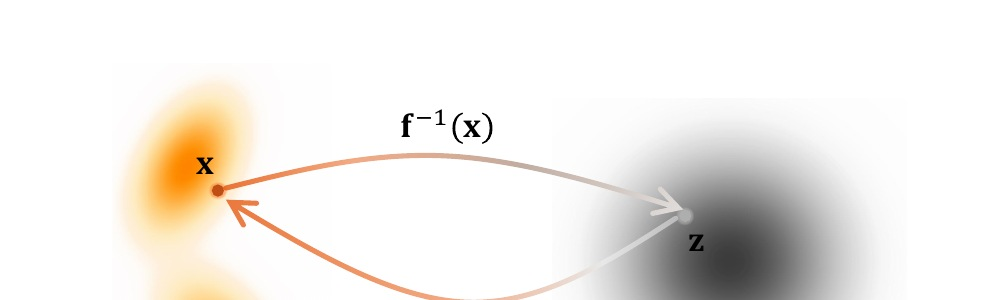
\includegraphics[width=\textwidth,height=0.58\textheight,keepaspectratio]{fig-5-2.jpg}
    \vfill
    \footnotesize
    $\bm{f}:\bm{z}\mapsto\bm{x}$（生成）と$\bm{f}^{-1}:\bm{x}\mapsto\bm{z}$（正規化）。\\
    密度の変化は変数変換公式で計算できる。
\end{frame}
%=============================================
\asmain
\begin{frame}{正規化フローの定義}
    単純な事前$p_{\mathrm{prior}}(\bm{z})$（例：$\mathcal{N}(\bm{0},\bm{I})$）を、\\
    可逆写像$\bm{f}_\phi:\mathbb{R}^{D}\to\mathbb{R}^{D}$で運ぶ：
    \[
        \bm{x}=\bm{f}_\phi(\bm{z}),
        \qquad
        \bm{z}\sim p_{\mathrm{prior}}
    \]
    変数変換より尤度は
    \[
        \log p_\phi(\bm{x})
        =
        \log p_{\mathrm{prior}}(\bm{z})
        +
        \log\det
        \dfrac{\partial\bm{f}_\phi^{-1}(\bm{x})}{\partial\bm{x}}
        \tag{5.1.1}
    \]
    学習は最尤
    $\mathcal{L}_{\mathrm{NF}}(\phi)=\mathbb{E}_{\bm{x}\sim p_{\mathrm{data}}}[\log p_\phi(\bm{x})]$
    （式5.1.2）。
\end{frame}
%=============================================
\asmain
\begin{frame}{図5.3：可逆層の積み重ね}
    \centering
    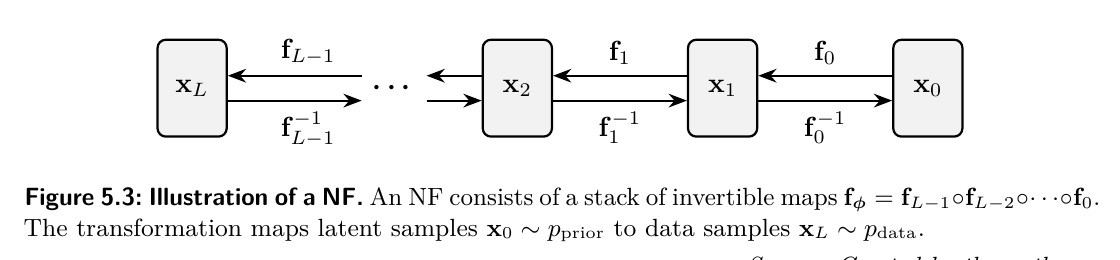
\includegraphics[width=\textwidth,height=0.48\textheight,keepaspectratio]{fig-5-3.jpg}
    \vfill
    \footnotesize
    $\bm{f}_\phi=\bm{f}_{L-1}\circ\cdots\circ\bm{f}_0$。\\
    $\bm{x}_0\sim p_{\mathrm{prior}}$を$\bm{x}_L\sim p_{\mathrm{data}}$へ運ぶ。
\end{frame}
%=============================================
\asmain
\begin{frame}{積み重ねとログ密度}
    各層$\bm{x}_{k+1}=\bm{f}_k(\bm{x}_k)$（式5.1.3）について
    \[
        \log p_\phi(\bm{x})
        =
        \log p_{\mathrm{prior}}(\bm{x}_0)
        +
        \sum_{k=0}^{L-1}
        \log\det
        \dfrac{\partial\bm{f}_k^{-1}}{\partial\bm{x}_k}
        \tag{5.1.4}
    \]
    \begin{block}{設計のトレードオフ}
        1層で複雑な可逆ネット$\Rightarrow$ヤコビアンが重い。\\
        単純な可逆層を多く積む$\Rightarrow$各層の$\det$は安く、表現力は積で稼ぐ。
    \end{block}
\end{frame}
%=============================================
\assuppl
\begin{frame}{\supplmark：代表的な可逆層}
    \begin{columns}[T,onlytextwidth]
        \begin{column}{0.48\textwidth}
            \begin{exampleblock}{Planar Flow}
                $\bm{f}(\bm{z})=\bm{z}+\bm{u}\,h(\bm{w}^{\top}\bm{z}+b)$\\
                $\det$はスカラー形で安い。
            \end{exampleblock}
        \end{column}
        \begin{column}{0.48\textwidth}
            \begin{exampleblock}{Residual Flow}
                $\bm{f}(\bm{z})=\bm{z}+\bm{v}(\bm{z})$（式5.1.5）\\
                収縮なら可逆。\\
                $\log\det$はトレース展開（5.1.6）。
            \end{exampleblock}
        \end{column}
    \end{columns}
    \vspace{0.35em}
    \begin{exampleblock}{次への橋}
        残差更新$\bm{x}+\bm{v}(\bm{x})$を細かく刻むと、連続時間のODEに近づく。
    \end{exampleblock}
\end{frame}
%=============================================
\asmain
\begin{frame}{図5.4：離散NFと連続NF}
    \centering
    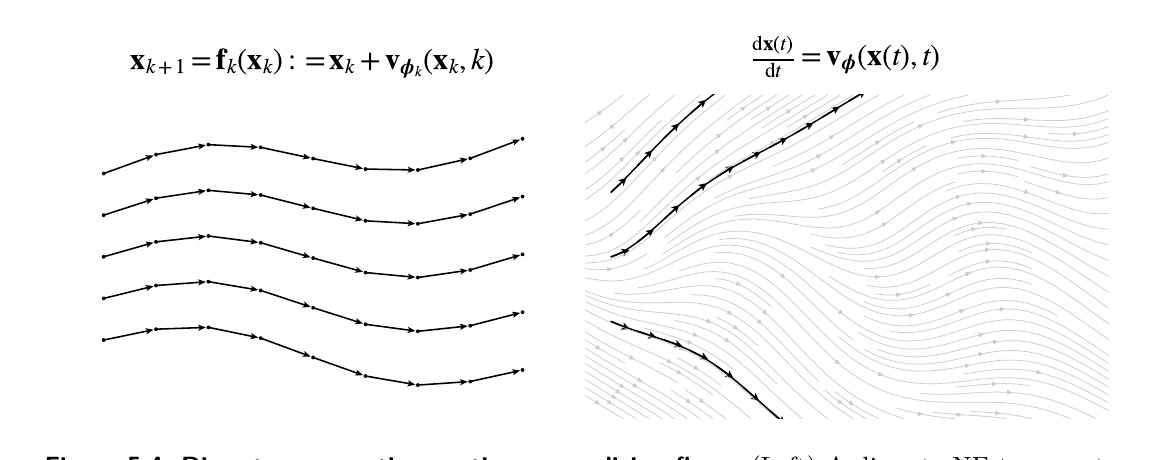
\includegraphics[width=\textwidth,height=0.58\textheight,keepaspectratio]{fig-5-4.jpg}
    \vfill
    \footnotesize
    左：有限個の可逆写像（点と矢印）。\\
    右：速度場に沿う積分曲線（Neural ODE）。
\end{frame}
%=============================================
\asmain
\begin{frame}{NFのまとめ}
    \begin{itemize}
        \item 可逆写像で事前$\leftrightarrow$データ。尤度は変数変換（5.1.1）（5.1.4）
        \item 表現力は層の積み重ねで稼ぎ、各層のヤコビアンは軽く保つ
        \item 残差型の細かい更新は、連続時間の速度場へ自然につながる
    \end{itemize}
    \begin{block}{次}
        $\Delta t\to 0$の極限としてNeural ODEを書く。
    \end{block}
\end{frame}
%=============================================
\section{Neural ODEs}
\asmain
\begin{frame}{区切り：Neural ODEs}
    \tableofcontents[currentsection]
\end{frame}
%=============================================
\asmain
\begin{frame}{離散層から連続時間へ}
    各層を小さな残差更新とみなす：
    \[
        \bm{x}_{k+1}
        =
        \bm{x}_k
        +
        \Delta t\,\bm{v}_\phi(\bm{x}_k,t_k),
        \qquad
        t_k=k\Delta t,\quad
        \Delta t=\dfrac{T}{L}
    \]
    $L\to\infty$、$\Delta t\to 0$で
    \[
        \dfrac{d\bm{x}(t)}{dt}
        =
        \bm{v}_\phi(\bm{x}(t),t),
        \qquad
        t\in[0,T]
        \tag{5.1.7}
    \]
    \begin{block}{呼び名}
        Neural ODE／Continuous Normalizing Flow。\\
        時刻の約束：$t=0$が事前、$t=T$（または$1$）がデータ。
    \end{block}
\end{frame}
%=============================================
\asmain
\begin{frame}{図5.5：離散双射から連続輸送へ}
    \centering
    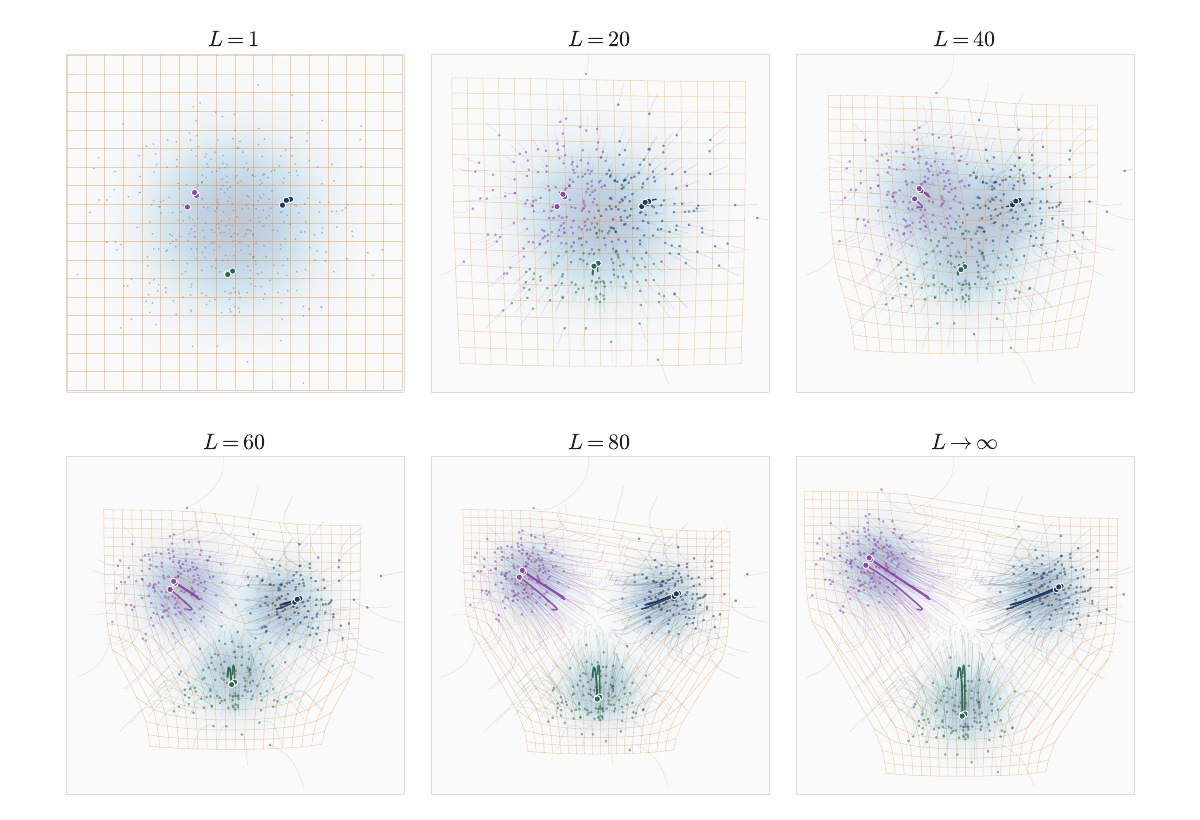
\includegraphics[width=\textwidth,height=0.62\textheight,keepaspectratio]{fig-5-5.jpg}
    \vfill
    \footnotesize
    $L$を増やすと、サンプル軌跡と格子変形が滑らかになる。\\
    $L\to\infty$で時間依存の連続流に近づく。
\end{frame}
%=============================================
\assuppl
\begin{frame}{\supplmark：図5.5の読み方}
    \begin{itemize}
        \item 色付き点：事前（ガウス）から3峰の目標へ運ばれるサンプル
        \item 橙の格子：空間の変形（体積の伸び縮み）を可視化
        \item $L$が小さい：各層の変形が大きい／粗い
        \item $L\to\infty$：軌跡が滑らかな曲線になり、速度場の積分曲線に見える
    \end{itemize}
    \begin{exampleblock}{密度側}
        運ばれた密度の時間発展は連続の方程式（式5.2.8）に従う。
    \end{exampleblock}
\end{frame}
%=============================================
\asmain
\begin{frame}{瞬間の変数変換公式}
    ODE軌道に沿って
    \[
        \dfrac{d}{dt}\log p_\phi(\bm{x}(t),t)
        =
        -\nabla_{\bm{x}}\cdot\bm{v}_\phi(\bm{x}(t),t)
    \]
    $t=0\to T$で積分すると
    \[
        \log p_\phi(\bm{x}(T),T)
        =
        \log p_{\mathrm{prior}}(\bm{x}(0))
        -
        \int_0^{T}
        \nabla_{\bm{x}}\cdot\bm{v}_\phi(\bm{x}(t),t)\,dt
        \tag{5.1.8}
    \]
    \begin{block}{離散との対応}
        和$\sum_k\log\det$が積分$\int(-\nabla\cdot\bm{v})\,dt$に置き換わる。
    \end{block}
\end{frame}
%=============================================
\assuppl
\begin{frame}{\supplmark：補題5.1.1（瞬間の変数変換）}
    ODE $\dfrac{d\bm{z}(t)}{dt}=\bm{F}(\bm{z}(t),t)$ に従う過程について、\\
    十分正則なら軌道に沿って
    \[
        \dfrac{d}{dt}\log p(\bm{z}(t),t)
        =
        -\nabla_{\bm{z}}\cdot\bm{F}(\bm{z}(t),t)
        \tag{5.1.9}
    \]
    \begin{exampleblock}{見方}
        連続の方程式＋連鎖律の「軌道版」。\\
        拡散なしのFokker--Planck（連続の方程式）とつながる。
    \end{exampleblock}
\end{frame}
%=============================================
\asmain
\begin{frame}{NODEの学習と推論}
    \begin{block}{学習（最尤）}
        $\mathcal{L}_{\mathrm{NODE}}(\phi)
        =\mathbb{E}_{\bm{x}\sim p_{\mathrm{data}}}[\log p_\phi(\bm{x},T)]$。\\
        データ$\bm{x}$から逆向きにODEを解き、発散を積分（式5.1.10）。
    \end{block}
    \begin{block}{推論（サンプリング）}
        $\bm{x}(0)\sim p_{\mathrm{prior}}$を前向き積分：
        \[
            \bm{x}(T)
            =
            \bm{x}(0)
            +
            \int_0^{T}\bm{v}_{\phi^\star}(\bm{x}(t),t)\,dt
        \]
    \end{block}
    \begin{alertblock}{実務上の課題}
        学習ループ内でODEを繰り返し解く必要があり、計算が重い。
    \end{alertblock}
\end{frame}
%=============================================
\asmain
\begin{frame}{連続の方程式への直感}
    速度場$\bm{v}_t$が密度$p_t$を運ぶとき、質量保存は
    \[
        \partial_t p_t(\bm{x})
        +
        \nabla\cdot\bigl(\bm{v}_t(\bm{x})\,p_t(\bm{x})\bigr)
        =
        0
    \]
    （連続の方程式；論文では式5.2.8）。
    \begin{itemize}
        \item NODE／PF-ODE：粒子は$\dot{\bm{x}}=\bm{v}_t(\bm{x})$で動く
        \item 密度側：上式で$\{p_t\}$が決まる
        \item 図5.5の「格子の変形」は、この輸送の幾何的イメージ
    \end{itemize}
\end{frame}
%=============================================
\asmain
\begin{frame}{NODEのまとめ}
    \begin{itemize}
        \item 離散NFの残差更新$\to$連続ODE（5.1.7）
        \item 尤度は発散の時間積分（5.1.8）
        \item 生成はODEの数値積分；学習もソルバが要り高い
    \end{itemize}
    \begin{block}{問い（Question 5.1.1）}
        学習中にODEを何度も解かずに、速度場をどう学ぶか？
    \end{block}
\end{frame}
%=============================================
\asmain
\begin{frame}{5.1 全体のまとめ}
    \begin{enumerate}
        \item \textbf{NF}
        可逆写像＋変数変換で尤度評価（5.1.1）（5.1.4）
        \item \textbf{積み重ね}
        軽い可逆層の合成で表現力を稼ぐ（図5.3）
        \item \textbf{NODE}
        連続極限の速度場（5.1.7）と瞬間の変数変換（5.1.8）
        \item \textbf{橋}
        スコア$\to$速度ではなく、速度を直接学ぶ動機が立つ
    \end{enumerate}
\end{frame}
%=============================================
\asmain
\begin{frame}{5.1 全体のまとめ：一本の流れ}
    \begin{block}{今日の道筋}
        可逆写像（NF）
        $\;\to\;$
        残差の連続極限（NODE）
        $\;\to\;$
        「ODEなしで速度を学ぶ」へ
    \end{block}
    \begin{block}{核心}
        生成＝確率分布を運ぶ速度場の学習。\\
        NODEは尤度積分で学ぶが、シミュレーションがボトルネック。
    \end{block}
    \begin{block}{次へ}
        5.2ではFlow Matching：条件付き速度への回帰で、\\
        周辺速度をシミュレーションフリーに学ぶ。
    \end{block}
\end{frame}
